\begin{figure}[H]
\centering
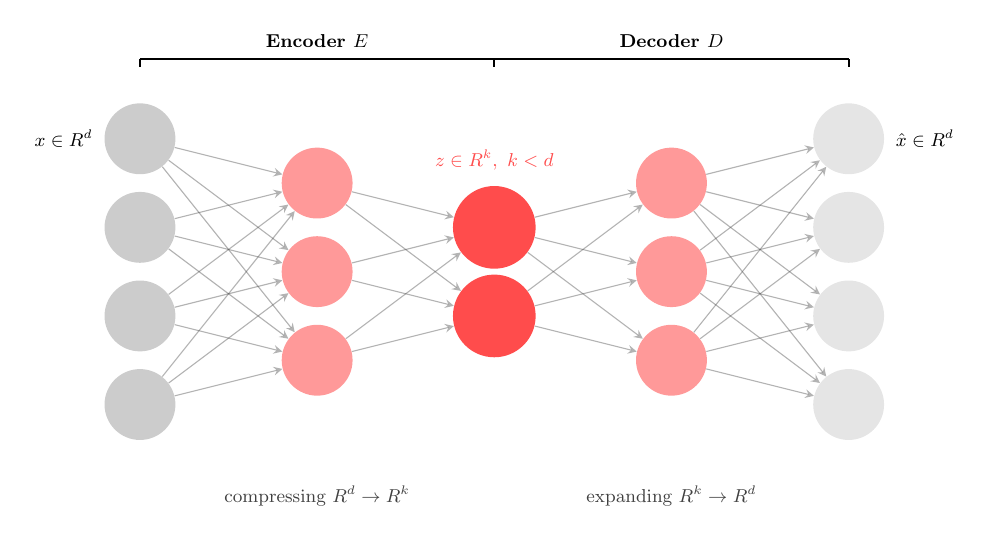
\begin{tikzpicture}[
    scale=0.75,
    transform shape,
    neuron/.style={circle, minimum size=12mm, inner sep=0pt},
    >=stealth
]
\definecolor{darkgrey}{RGB}{90,90,90}

% ======================
% Input layer: 4 nodes
% ======================
\node[neuron, fill=gray!40] (I1) at (0,  2.25) {};
\node[neuron, fill=gray!40] (I2) at (0,  0.75) {};
\node[neuron, fill=gray!40] (I3) at (0, -0.75) {};
\node[neuron, fill=gray!40] (I4) at (0, -2.25) {};

% ======================
% Encoder hidden: 3 nodes
% ======================
\node[neuron, fill=red!40] (E1) at (3,  1.5) {};
\node[neuron, fill=red!40] (E2) at (3,  0.0) {};
\node[neuron, fill=red!40] (E3) at (3, -1.5) {};

% ======================
% Latent: 2 nodes
% ======================
\node[neuron, fill=red!70, minimum size=14mm] (Z1) at (6,  0.75) {};
\node[neuron, fill=red!70, minimum size=14mm] (Z2) at (6, -0.75) {};

% ======================
% Decoder hidden: 3 nodes
% ======================
\node[neuron, fill=red!40] (D1) at (9,  1.5) {};
\node[neuron, fill=red!40] (D2) at (9,  0.0) {};
\node[neuron, fill=red!40] (D3) at (9, -1.5) {};

% ======================
% Output layer: 4 nodes
% ======================
\node[neuron, fill=gray!20] (O1) at (12,  2.25) {};
\node[neuron, fill=gray!20] (O2) at (12,  0.75) {};
\node[neuron, fill=gray!20] (O3) at (12, -0.75) {};
\node[neuron, fill=gray!20] (O4) at (12, -2.25) {};

% ======================
% Connections input → enc hidden
% ======================
\foreach \s in {I1,I2,I3,I4} {
    \foreach \t in {E1,E2,E3} {
        \draw[->, draw=darkgray, opacity=0.4] (\s) -- (\t);
    }
}

% ======================
% Connections enc hidden → latent
% ======================
\foreach \s in {E1,E2,E3} {
    \foreach \t in {Z1,Z2} {
        \draw[->, draw=darkgray, opacity=0.4] (\s) -- (\t);
    }
}

% ======================
% Connections latent → dec hidden
% ======================
\foreach \s in {Z1,Z2} {
    \foreach \t in {D1,D2,D3} {
        \draw[->, draw=darkgray, opacity=0.4] (\s) -- (\t);
    }
}

% ======================
% Connections dec hidden → output
% ======================
\foreach \s in {D1,D2,D3} {
    \foreach \t in {O1,O2,O3,O4} {
        \draw[->, draw=darkgray, opacity=0.4] (\s) -- (\t);
    }
}

% ======================
% Node labels
% ======================
\node[left=2pt,  font=\small] at (I1.west) {$x \in \mathbb{R}^d$};
\node[right=2pt, font=\small] at (O1.east) {$\hat{x} \in \mathbb{R}^d$};
\node[above=4pt, font=\small, red!70] at (Z1.north) {$z \in \mathbb{R}^k,\ k < d$};

% ======================
% Encoder bracket
% ======================
\def\StepTick{4pt}
\def\BracketY{3.6}
\draw[thick] (0, \BracketY)  -- ++(0, -\StepTick);
\draw[thick] (0, \BracketY)  -- (6,  \BracketY);
\draw[thick] (6, \BracketY)  -- ++(0, -\StepTick);
\node[above=2pt, font=\small\bfseries] at (3, \BracketY) {Encoder $E$};

% ======================
% Decoder bracket
% ======================
\draw[thick] (6,  \BracketY) -- ++(0, -\StepTick);
\draw[thick] (6,  \BracketY) -- (12, \BracketY);
\draw[thick] (12, \BracketY) -- ++(0, -\StepTick);
\node[above=2pt, font=\small\bfseries] at (9, \BracketY) {Decoder $D$};

% ======================
% Bottom annotations
% ======================
\node[font=\small, darkgray] at (3,  -3.8) {compressing $\mathbb{R}^d \to \mathbb{R}^k$};
\node[font=\small, darkgray] at (9,  -3.8) {expanding $\mathbb{R}^k \to \mathbb{R}^d$};

\end{tikzpicture}
\caption{Undercomplete autoencoder with a symmetric encoder--decoder
architecture. The encoder $E$ compresses the input $x \in \mathbb{R}^d$
into a latent representation $z \in \mathbb{R}^k$ with $k < d$, and the
decoder $D$ reconstructs $\hat{x} \in \mathbb{R}^d$ from $z$.}
\label{fig:autoencoder}
\end{figure}